\input{setup/preamble.tex}% package inclusion and set up of the document

%%%%%%%%%%%%%%%%%%%%%%%%%%%%%%%%%%%%%%%%%%%%%%%%%%%%%
%             UNITS, EQUATIONS AND TEXT             %
%%%%%%%%%%%%%%%%%%%%%%%%%%%%%%%%%%%%%%%%%%%%%%%%%%%%%
%Units:
\newcommand{\unit}[1]{&& \left[\si{#1}\right]} %\newcommand{\unit}[1]{[\si{#1}]}             <<| Use these if you want equations to be
\newcommand{\unitWh}[1]{[\si{#1}]}             %\newcommand{\eq}[2]{&&\si{#1} &= \si{#2}&&}  <<| centered.. .. will appear scrambled
\newcommand{\numUnit}[1]{\ \si{#1}&}           %                                               | from one equation to the next though..
%Equation:                                     %                                               | and does not work with long equations.. :/
\newcommand{\eq}[2]{\si{#1} &= \si{#2}}
\newcommand{\arw}{&& &\Updownarrow&&}
%Text:
\newcommand{\tx}[1]{\text{#1}}
%Vectors
\renewcommand{\vec}[1]{\boldsymbol{\mathbf{#1}}}
%Vertical line in equations ie. |_x=y (whereTwo stacks two equalities at the line)
\newcommand{\where}[1]{ \left.\rule{0cm}{.5cm}\right\vert\rule{0cm}{.4cm}_{\substack{\rule{0cm}{.15cm}\\ \si{#1} }} }
\newcommand{\whereTwo}[2]{ \left.\rule{0cm}{.67cm}\right\vert\rule{0cm}{.5cm}_{\substack{\si{#1} \rule{0cm}{.19cm}\\\vspace{-.1cm}\\ \si{#2}}} }

%%%%%%%%%%%%%%%%%%%%%%%%%%%%%%%%%%%%%%%%%%%%%%%%%%%%%
%                  REFERENCES                       %
%%%%%%%%%%%%%%%%%%%%%%%%%%%%%%%%%%%%%%%%%%%%%%%%%%%%%

%Chapter
\newcommand{\Chapref}[1]{\emph{Chapter \ref{#1}}}
\newcommand{\chapref}[1]{\emph{chapter \ref{#1}}}
%Section
\newcommand{\Secref}[1]{\emph{Section \ref{#1}}}
\newcommand{\secref}[1]{\emph{section \ref{#1}}}
%subSection
\newcommand{\Subsecref}[1]{\emph{Subsection \ref{#1}}}
\newcommand{\subsecref}[1]{\emph{subsection \ref{#1}}}
%Appendix
\newcommand{\Appref}[1]{\emph{Appendix \ref{#1}}}
\newcommand{\appref}[1]{\emph{appendix \ref{#1}}}
%Listings
\newcommand{\Coderef}[1]{\emph{Listings: \ref{#1}}}
\newcommand{\coderef}[1]{\emph{listings: \ref{#1}}}
%Figure:
\newcommand{\Figref}[1]{\emph{Figure \ref{#1}}}
\newcommand{\figref}[1]{\emph{figure \ref{#1}}}
%Table:
\newcommand{\Tableref}[1]{\emph{Table \ref{#1}}}
\newcommand{\tableref}[1]{\emph{table \ref{#1}}}

%Expressions:
\newcommand{\Expr}[1]{\emph{Expression (\ref{#1})}}
\newcommand{\expr}[1]{\emph{expression (\ref{#1})}}

%Equations:
%1 equation:
\newcommand{\Eqref}[1]{\emph{Equation (\ref{#1})}}
\renewcommand{\eqref}[1]{\emph{equation (\ref{#1})}}
%2 equations:
\newcommand{\EqrefTwo}[2]{\emph{Equation (\ref{#1})} and \emph{(\ref{#2})}}
\newcommand{\eqrefTwo}[2]{\emph{equation (\ref{#1})} and \emph{(\ref{#2})}}
%3 equations:
\newcommand{\EqrefThree}[3]{\emph{Equation (\ref{#1})}, \emph{(\ref{#2})} and \emph{(\ref{#3})}}
\newcommand{\eqrefThree}[3]{\emph{equation (\ref{#1})}, \emph{(\ref{#2})} and \emph{(\ref{#3})}}
%4 equations:
\newcommand{\EqrefFour}[4]{\emph{Equation (\ref{#1})}, \emph{(\ref{#2})}, \emph{(\ref{#3})} and \emph{(\ref{#4})}}
\newcommand{\eqrefFour}[4]{\emph{equation (\ref{#1})}, \emph{(\ref{#2})}, \emph{(\ref{#3})} and \emph{(\ref{#4})}}
%5 equations:
\newcommand{\EqrefFive}[5]{\emph{Equation (\ref{#1})}, \emph{(\ref{#2})}, \emph{(\ref{#3})}, \emph{(\ref{#4})} and \emph{(\ref{#5})}}
\newcommand{\eqrefFive}[5]{\emph{equation (\ref{#1})}, \emph{(\ref{#2})}, \emph{(\ref{#3})}, \emph{(\ref{#4})} and \emph{(\ref{#5})}}
%6 equations:
\newcommand{\EqrefSix}[6]{\emph{Equation (\ref{#1})}, \emph{(\ref{#2})}, \emph{(\ref{#3})}, \emph{(\ref{#4})}, \emph{(\ref{#5})} and \emph{(\ref{#6})}}
\newcommand{\eqrefSix}[6]{\emph{equation (\ref{#1})}, \emph{(\ref{#2})}, \emph{(\ref{#3})}, \emph{(\ref{#4})}, \emph{(\ref{#5})} and \emph{(\ref{#6})}}
%7 equations:
\newcommand{\EqrefSeven}[7]{\emph{Equation (\ref{#1})}, \emph{(\ref{#2})}, \emph{(\ref{#3})}, \emph{(\ref{#4})}, \emph{(\ref{#5})}, \emph{(\ref{#6})} and \emph{(\ref{#7})}}
\newcommand{\eqrefSeven}[7]{\emph{equation (\ref{#1})}, \emph{(\ref{#2})}, \emph{(\ref{#3})}, \emph{(\ref{#4})}, \emph{(\ref{#5})}, \emph{(\ref{#6})} and \emph{(\ref{#7})}}% my new macros

\begin{document}
%%% Prereport %%%
\setlength\cftaftertoctitleskip{2pt}
\setlength\cftafterloftitleskip{6pt}
\setlength\cftafterlottitleskip{6pt}
\selectlanguage{english}
\title{Cubli}

%%% Frontmatter Settings %%%
\pagestyle{empty} %disable headers and footers
\pagenumbering{roman} %use roman page numbering in the frontmatter I II...
\fancyfoot[RE,LO]{16gr630} %page number on all pages
\fancyfoot[LE,RO]{\thepage}
\fancyhead[LE,LO,RE,RO]{}

%%% Introductory Formalities %%%
%\includepdf[pages={1}]{formalities/frontpage.pdf}
%\pdfbookmark[0]{Front Page}{label:forside}%
\begin{titlepage}
  \addtolength{\hoffset}{0.5\evensidemargin-0.5\oddsidemargin} %set equal margins on the frontpage - remove this line if you want default margins
  \noindent%
  \begin{tabular}{@{}p{\textwidth}@{}}
    \toprule[2pt]
    \midrule
    \vspace{0.2cm}
    \begin{center}
    \Huge{\textbf{
      Autonomous Lawn Mower % insert your title here
    }}
    \end{center}
    \begin{center}
      \Large{
      Utilizing a Local Positioning System
      }
    \end{center}
    \vspace{0.2cm}\\
    \midrule
    \toprule[2pt]
  \end{tabular}
   \vspace{0.55 cm}
  \begin{figure}[!ht]
\centering
\includegraphics[width=0.8\textwidth]{figures/frontPageImage.pdf}
\label{fig:forside}
\end{figure}
  \vspace{-0.35 cm}
  \begin{center}
    {\large
      5. Semester Project Report %Insert document type (e.g., Project Report)
    }\\
    \vspace{0.2cm}
    {\Large
      Group 15gr510%Insert your group name or real names here
    }
  \end{center}
  \begin{center}
  Aalborg University\\
  Electronic Engineering \& IT\\
  Fredrik Bajers Vej 7\\
  DK-9220 Aalborg
  \end{center}
\end{titlepage}

\clearpage
\pagestyle{fancy}
{\small
\strut\vfill % push the content to the bottom of the page
\noindent Copyright \copyright{} Aalborg University 2015\par
\vspace{0.2cm}

\noindent This report is compiled in \LaTeX, originally developed by Leslie Lamport, based on Donald Knuth's \TeX. The main text is written in \emph{Latin Modern} pt 12, designed by Bogusław Jackowski and Janusz M. Nowacki. 
%The document is compiled via the website \url{www.overleaf.com}, an online collaborative based \LaTeX-editor with instant preview, which enables multiple persons to edit the document simultaneously.
Flowcharts and diagrams are made using Microsoft Visio. 
\clearpage
%\begin{document} 
%\thispagestyle{empty}
%\begin{titlepage}
\begin{nopagebreak}
{\samepage 

\begin{tabular}{r}
\parbox{\textwidth}{  \raisebox{-15mm}{\includegraphics[height=3cm]{figures/aaulogo-en.png}}
\hfill \hspace{2cm} \parbox{8cm}{\begin{tabular}{l} %4.90
{\small \textbf{\textcolor{aaublue}{\colorbox{white}{6\textsuperscript{th} Semester, Bachelor Project}}}}\\
{\small \textbf{\textcolor{aaublue}{School of Information and}}}\\
{\small \textbf{\textcolor{aaublue}{Communication Technologies}}}\\ 
{\small \textbf{\textcolor{aaublue}{Electronics and IT}}}\\
{\small \textcolor{aaublue}{Fredrik Bajers Vej 7C}} \\
{\small \textcolor{aaublue}{9220 Aalborg}} \\
{\small \textcolor{aaublue}{\emph{http://www.sict.aau.dk/electronics-and-it}}}
\end{tabular}}}
\end{tabular}

\begin{tabular}{cc}
\parbox{7cm}{

\textbf{Title:}

Cubli:\\
Dynamic Control of a Reaction Wheel Inverted Pendulum\\ %\fxnote{Input project title}\\

\textbf{Theme:}

\small{
BSc Project (Control Engineering)\\
}


\parbox{8cm}{


\textbf{Project Period:}\\
P6, Spring 2016\\
01/02/2016 - 25/05/2016\\
   
\textbf{Project Group:}\\
630\\ %\fxnote{Input group number}
  
\textbf{Participants:}\\
Bjørn Kitz\\
Julien Br\'ehin\\
Mikael Sander\\
Niels Skov Vestergaard\\
Noelia Villarmarzo Arruñada\\

\textbf{Supervisors:}\\
John-Josef Leth\\ %\fxnote{Input supervisor}
Palle Andersen
}\\

\textbf{Prints:} 8\\
\textbf{Pages:} 125\\
\textbf{Appendices:} 15 (37 pages)\\
\textbf{Attached:} 1 DVD\\
\textbf{Concluded:} 25/05/2016\\

\vfill } &
\parbox{7cm}{
  \vspace{.15cm}
  \hfill
  \begin{tabular}{l}
  {\textbf{Synopsis}}\bigskip \\
  \fbox{
    \parbox{6.5cm}{\bigskip
     {\vfill{\small The inverted pendulum is used in many applications and it is a classic research area in control theory which is still active.

The aim of this project was to model and analyze the behavior of a reaction wheel inverted pendulum, in the form of a one-frame Cubli; and to design a controller capable of balancing it in equilibrium position. 

A controller was designed using classical control methods such as root locus and Nyquist criterion. However, the system had a marginally stable behavior. Not having control of the velocity of the reaction wheel was a problem, so the final controller was done through state space design.

Moreover, a solution for measuring its angular position using only internally mounted sensors was designed to be able to make it portable to a full Cubli. 

Finally, the performance of the system was tested on the prototype to ensure that it fulfills the needed requirements.
     \bigskip}}
     }}
   \end{tabular}}
\end{tabular}} %\vspace{1cm}

\textit{\phantom{A}Publication of this report's contents (including citation) without permission\\ \phantom{A}from the authors is prohibited}\\

\end{nopagebreak}
%\end{titlepage}
%\end{document}
%%% Preface %%%
%\cleardoublepage
\textbf{\huge{Preface}}
\\
\\
The purpose of this project is to design and implement a control system that can maintain a reaction wheel inverted pendulum in upright position using only internally mounted sensors.

This report has been written by a group of students on the sixth semester of "Electronics and IT" at Aalborg University.
The reader should have a basic knowledge on Electronic Engineering, specially in Modeling and Control Theory, and Convex Optimization, although specific topics will be described in more detail. Code for the implementation is written in C++ and the reader is assumed to be able to comprehend this programming language. 

Thanks:\\
- Simon Jensen, assistant engineer, Department of Electronic Systems, Aalborg University \\
- Simon Vestergaard Johansen, Business Ph.d., worked with the cubli previously, discussed project with us,\\
- Benjamin Krebs, former AAU student, wrote the base code for the cubli, has provided help.\\
- Thanks to our supervisors John-Josef Leth and Palle Andersen

\textbf{Reading Instructions}
\\
\\
The report is structured in three parts:
\begin{itemize}
\item[-] Part I contains an analysis of the system, which includes a description of the given setup, the derivation of the dynamic model and the acquisition of the parameters of the system.
\item[-] Part II deals with the design and implementation of the controller and the complementary filter used to measure the angular position of hte frame.
\item[-] Part III includes the acceptance tests made to the system and the conclusions that can be derived from the project.
\end{itemize}

The attached CD contains a digital copy of this report, all the data and Matlab files needed to plot the figures in the report, datasheets, the code needed to run the controller, the code needed for the implementation of the optimization, the Senstools manual and a video of the working system.  

\textbf{Text by:}\\
\vspace{-12 pt}
\begin{table}[H]
	\centering
		\begin{tabular}{c c c}
			\underline{\phantom{JAERJAERJAERJAERGO}} & \phantom{cookies} & \underline{\phantom{JAERJAERJAERJAERGO}} \\
			Bjørn Kitz			& \phantom{cookies} & Julien Br\'ehin		\\
			&&\\
			\underline{\phantom{JAERJAERJAERJAERGO}} & \phantom{cookies} & \underline{\phantom{JAERJAERJAERJAERGO}} \\
			Mikael Sander			& \phantom{cookies} & Niels Skov Vestergaard		\\
			&&\\
	    \multicolumn{3}{c}{\underline{\phantom{JAERJAERJAERJAERGO}}}\\
	    \multicolumn{3}{c}{Noelia Villarmarzo Arruñada}\\				
		\end{tabular}
\end{table}
\pagebreak

\pdfbookmark[0]{Table of Contents}{label: tableOfCentents}
\tableofcontents
\cleardoublepage


%%% Mainmatter Settings %%%
\pagenumbering{arabic} %use arabic page numbering in the mainmatter
\fancyfoot[RO,LE]{\thepage \text{ of} \pageref{LastPage}}
\fancyfoot[RE,LO]{16gr630}
\fancyhead[RE,LO]{}
\fancyhead[RE,LO]{\color{aaublue}\small\nouppercase\leftmark} %even page - chapter title
\pagestyle{fancy}

%%% Part 1 %%%
\part{Preanalysis}

%---------- Chapter 1 ---------------------------------------- Introduction
\chapter{Introduction}\label{introduction}
The effective control of an inverted pendulum is still an active area of research nowadays. \cite{JHuber}

One type of this kind of systems is a setup called Cubli. It consists of a cube controlled with reaction wheels. The Cubli can jump up and balance on one of its edges or on one of its corners, as shown in \figref{CubliCorner}.
The Cubli is designed as a simple setup to let control engineers work with an inverted pendulum. A working Cubli can also be an interesting way to show and explain the general public  what control engineering is about. \cite{MGajamohan}
%
\begin{figure}[H] 
	\centering
	\includegraphics[scale=1.3]{figures/CubliCorner-700x430}
	\caption{A Cubli balancing on one of its corners\cite{RAndrea}}
	\label{CubliCorner}
\end{figure}
%
Applications for this cube robot, that moves without any external tools, might seem limited when you only have a single cube. However, if you take a group of cubes, they could move together to traverse obstacles or solve puzzles one cube alone could not. A group of cubes can form a structure (\figref{MBlocksExample}), and by talking in between each other they can use their reaction wheels to get the structure to move in the desired direction. Since each cube can move independently, a single cube can detach for an assignment or catch up with the main structure if it gets dropped. \cite{JRomanishin}
%
\begin{figure}[H] 
	\centering
	\includegraphics[scale=0.4]{figures/m-blocks}
	\caption{A number of cube robots (called M-blocks at Massachusetts Institute of Technology (MIT)) shown making two different structures. These M-blocks stick together with the help of magnets placed in their corners \cite{LRosen}}
	\label{MBlocksExample}
\end{figure}
%
It has also been suggested using similar technology for alternative locomotion in planetary or asteroid exploration. The internal actuation is not very efficient in high gravity environments, however, in environments with microgravity such as asteroids the technology becomes very feasible. \cite{RAllen}

In microgravity a Cubli could tumble or even jump across the surface. A traditional rover with wheels would not be able to sufficiently grip or might even push the rover off the surface long enough for it to land upside down. Where such a situation would be fatal for most rovers, a cube with internal actuation would not be immobilized by landing upside down.\cite{ELandau}

This concept was the basis of a small experimental lander called MINERVA, short for Micro/Nano Experimental Robot Vehicle for Asteroids, which were to explore the near earth asteroid Itokawa (see \figref{MINERVA}). The lander was deployed from its mother spacecraft HAYABUSA in 2005, when it unfortunately missed the asteroid's small gravitational pull and drifted off into space. \cite{TYoshimitsu}
%
\begin{figure}[H] 
	\centering
	\includegraphics[scale=.8]{figures/MINERVA}
	\caption{MINERVA experimental lander, which was designed for asteroid exploration \cite{TYoshimitsu}}
	\label{MINERVA}
\end{figure}
%
A more recent example of development in this area is NASA's Hedgehog robot, which also is actuated internally with reaction wheels. It has bee through several tests aboard an aircraft for microgravity research in June 2015, where it showed its ability to jumping out of a sandpit. A picture of the Hedgehog robot can be seen in \figref{Hedgehog}. \cite{ELandau}
%
\begin{figure}[H] 
	\centering
	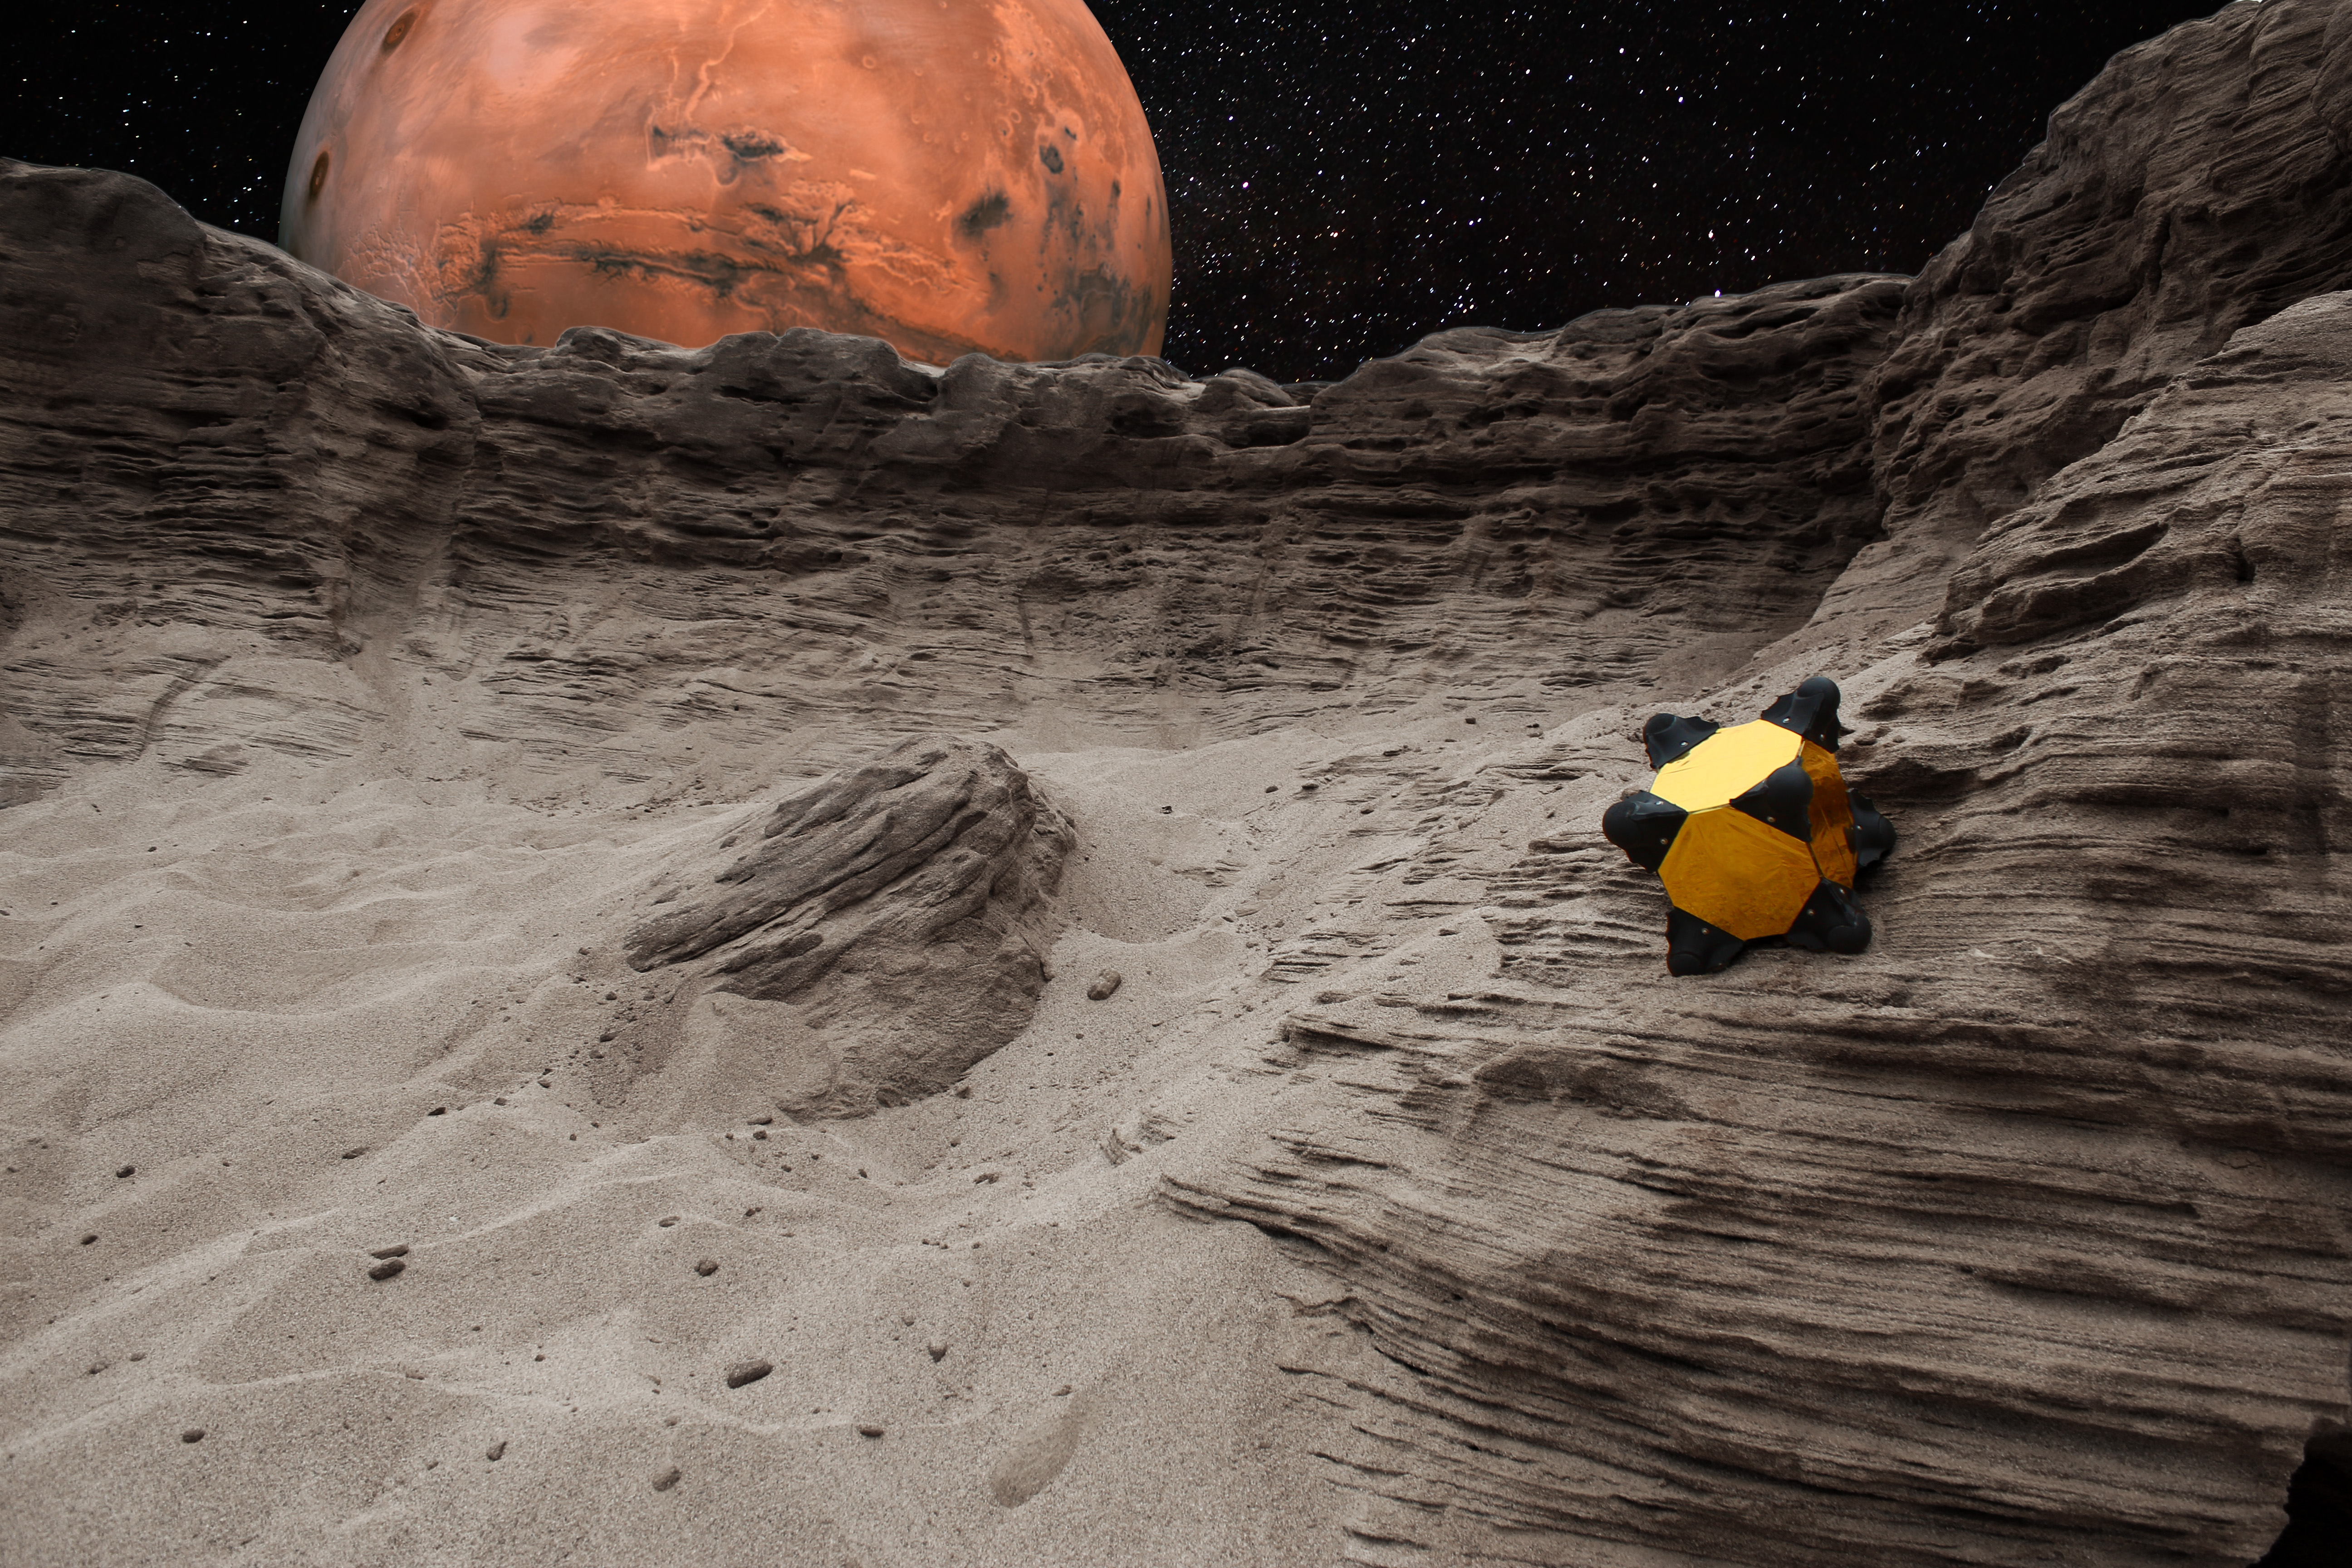
\includegraphics[scale=0.05]{figures/Hedgehog}
	\caption{NASA's Hedgehog robot for asteroid exploration \cite{ELandau}}
	\label{Hedgehog}
\end{figure}
%\section{AAU Cubli}
Here at AAU there was build a one-dimensional model of the cubli. It is fixed to an axis with one of its corners, so it can rotate around that corner, but cannot be moved translational.

The AAU cubli consists of the following parts\fxnote{insert correct part names}.

\begin{table}[H]
	\begin{tabular}{|l|p{3.8cm}|}
		\hline %-----------------------------------------------------------------------------------
		\textbf{No.} &\textbf{Part} 			\\
		\hline %-----------------------------------------------------------------------------------
		1            & Frame           			\\
		\hline %-----------------------------------------------------------------------------------
		2            & Reaction wheel      		\\
		\hline %-----------------------------------------------------------------------------------
		3            & IMU           			\\
		\hline %-----------------------------------------------------------------------------------
		4            & BeagleBone           	\\
		\hline %-----------------------------------------------------------------------------------
		5            & Potentiometer           	\\
		\hline %-----------------------------------------------------------------------------------
		6            & Motorcontrolboard    	\\
		\hline %-----------------------------------------------------------------------------------
		7            & Brushless DC-motor    	\\
		\hline %-----------------------------------------------------------------------------------
		8            & Jump brake		    	\\
		\hline %-----------------------------------------------------------------------------------
	\end{tabular}
	\caption{Table over parts in the Cubli setup \label{TableAAUCubliComponent}}
\end{table}

\subsection{Subsection 1.1.1}
The frame is made of metal? \fxnote{find composition of frame if possible} and is mainly a square with a solid edge at the outer bound of the frame, and two cross connections between opposing corners. 

The reaction wheel is a wheel made of metal? \fxnote{find composition of wheel if possible} with most of the mass in a ring at its outer edge and two crossconnections, that are going trough its center at rigth angle to each other. It is connected with the motor and the frame through and axis going throught its center of rotation.


The BeagleBone recieves the data from sensors and motor and with the control algorithm uploaded to it, tries to balance the cubli, by spinning up the reaction wheel.

The potentiometer is placed at the corner of the frame that is fixed to an axis. It is used to measure the angel of the frame.

The motor spins up the reaction wheel and also brakes it during the balancing part of the controller. When jumping up the cubli the motor will spin up the reaction wheel and the jump brake will then suddenly brake the reaction wheel.
\subsection{Subsection 1.1.2}
%\input{chapters/chapter1/cSectionAndSubsections.tex} %-------- For Overview, sometimes short headlines here works well

%---------- Chapter 2 ---------------------------------------- Design Considerations
\chapter{Design Considerations}
The setup for this project is given by the university, which means that some considerations must be taken into account when modeling the system and designing a controller to balance it.

%---------- Chapter 3 ---------------------------------------- Design Limitations
\section{Design Limitations}
The working setup that exists at Aalborg University (AAU) is composed by one of the sides of the 3D cube.

Since all the hardware is already build, the goal of the project is focus on deriving the model of the system, simulate it to compare it with the real Cubli and design a controller capable of balance it in the equilibrium position.

One important characteristic is that one of its corners is attached to a base plate. This feature limits the number of movements the Cubli can do, as it can only be balance in one direction.

Another important limitation is given by the maximum current that the motor can provide which conditions the maximum starting angle that it can have with respect to equilibrium position. As can be seen in \figref{}, if the initial angle is different from 0 rad both the mass of the frame ans the mass of the wheel exert an initial torque to the system. This must be overcame by the motor in order to the Cubli not to fall.
%
\begin{figure}[H] 
	\centering
	\includegraphics[scale=0.65]{figures/limitationTorque}
	\caption{Force acting on the system that create an initial torque}
	\label{limitationTorque}
\end{figure}

The minimum torque that the motor must apply is give by \eqref{minTorque}.
%
\begin{flalign}
	\eq{T} { (m_F \cdot l_F + m_w \cdot l_w) \cdot g \cdot sin(\theta_F)} \unit{N\cdot m}
	\label{minTorque}
\end{flalign}

Since the torque is restricted by the characteristics of the motor and the control board, the maximum initial angle is derived in \eqref{maxAngle}.
%
\begin{flalign}
	\eq{\theta_F} { asin\left(\frac{T}{(m_F \cdot l_F + m_w \cdot l_w) \cdot g}\right)} \unit{N\cdot m}
	\label{maxAngle}
\end{flalign}
%
Substituding the values of the maximum torque (see section \ref{sec:Motor}) and the parameters of the Cubli (see section \ref{sec:Param}) the maximum starting angle is \si{0,2024\ rad}.

\fxnote{The maximum angle may should be explained after the modeling and the estimation of parameters}
%At Aalborg University (AAU), there exists a working setup of a one-dimensional Cubli. The overall goals of this semester are to make a model of a system, to simulate this model and then to design and implement a controller for that system. Students on this semester are encouraged to work with pre-made setups, since the focus is rather on the control engineering than the hardware solution.\fxnote{moved the section directly from introduction. Will need a top to catch the previous chapter}



%---------- Chapter 4 ---------------------------------------- System Description
\chapter{System Description}\label{systemDescription}
One-frame Cubli is a non-linear unstable system which is capable of laying on one of its corners as long as it is properly controlled, using the inertia created in the reaction wheel present in the setup.



This system is composed by several hardware parts, listed in the following table. \fxnote{Include picture of the real model, mark all the parts in the picture}

\begin{table}[H]
	\begin{tabular}{|l|p{6.7cm}|}
		\hline %-----------------------------------------------------------------------------------
		\textbf{No.} &\textbf{Part} 			\\
		\hline %-----------------------------------------------------------------------------------
		1            & Frame           			\\
		\hline %-----------------------------------------------------------------------------------
		2            & Reaction wheel      		\\
		\hline %-----------------------------------------------------------------------------------
		3            & BeagleBone Black (microcontroller)  \\
		\hline %-----------------------------------------------------------------------------------
		4            & Potentiometer			\\
		\hline %-----------------------------------------------------------------------------------
		5            & Inertia Measurement Units (IMU)       			\\
		\hline %-----------------------------------------------------------------------------------
		6            & Brushless DC-motor   	\\
		\hline %-----------------------------------------------------------------------------------
		7            & Motor control board     	\\
		\hline %-----------------------------------------------------------------------------------
		8            & Jump brake (servomotor)		    	\\
		\hline %-----------------------------------------------------------------------------------
		9            & Connecting and breakout board		    	\\
		\hline %-----------------------------------------------------------------------------------
	\end{tabular}
	\caption{Main parts of the Cubli setup}
\label{TableAAUCubliComponent}
\end{table}

BeagleBone Black and Maxon motor control board and Maxon motor and break servomotor is mounted to the frame. On the motor shaft a freewheel is mounted. 

There is 2 pieces of IMU mounted on the frame. The IMU measures acceleration and angular velocity. The frame is mounted on the platform by a potentiometer so the angle of the frame can be measured.

To connect the BeagleBone Black to the other units like the Maxon motor control board and the IMU and potentiometer there is a connecting and breakout board.

The Cubli is a complete finish mechanical electronic system and have been built by others. From the previous groups that have been working on the Cubli some of the parameters have been found. To confirm and investigate the configuration of the mechanical parts changes has been made to the Cubli and the new parameters has not been measured and verified.


\section{Mechanical Components}
The mechanical part of the whole Cubli is composed of two important elements, which are the main components of a reaction wheel inverted pendulum: the frame and the reaction wheel.

\subsection{Frame}
The frame is made of aluminum with dimensions 17x16x0,5 \si{cm}  with two cross connections between opposing corners. The frame mounting is centered around the middle of the frame.
To keep the weight down on the frame, a large area of the frame is milled out. That composes the body of the Cubli. 

As it can only be balanced in one direction, it is attached to the base on one of its vertices to avoid it from falling in any of the other directions.

%It plays an important role since it acts like the inverted pendulum of the system and, moreover, all the electronics and the motor needed are attached to it.\fxnote{Isn't the motor rather attached to the wheel (both in reality and in the model) ? J.}
%This last aspect has to be taken into account when finding the model, as its moment of inertia, center of gravity and mass change.

\subsection{Reaction Wheel}
%A reaction wheel is a device used in many applications, such as attitude control in spacecrafts, when a change in rotation or keeping a certain attitude is needed.\fxnote{source?}
%The use of this kind of wheels allows these small variations in the rocket orientation, and thus reducing fuel needed to do this task.\fxnote{Do we really want a comparison with rockets or satellites?}
In the particular case of the Cubli, the reaction wheel is made of brass with most of the mass in a ring at its outer edge and two cross connections through its center.

The reaction wheel is coupled to the axis of a motor, through its center of rotation. When the wheel turns, its change of velocity creates a torque on the system that is transmitted with opposite direction to the body due to the conservation of angular momentum.		%-------- Mechanical Components
\section{Microcontroller - BeagleBone Black}

The microcontroller used on this system is a BeagleBone Black, which is in charge of managing the data from the motor and the sensors and of calculating the required control action.\\
It uses an ARM processor at a clock frequency of \SI{1}{GHz} and has a large amount of general purpose inputs and outputs, of which some of them support the I2C protocol or include an Analogue to Digital Converter (ADC).\\
In order to use the data from the potentiometer it has to be sampled by the ADC in  the BeagleBone. 
The ADCs of the BeagleBone have a 12-bit resolution that is limited to a range of \si{0 - 1,8 V}. The fastest sampling time it can provide is 125ns\cite{Cameon}.				      %-------- Controller
\section{Motor}
\label{sec:Motor}


\subsection{Brushless DC-Motor}
The brushless motor (EC 45 flat, 251601) can take a nominal current of 2.33 A.\cite{MaxonMotors} \fxnote{make sure the correct motor is listed and that the current is correct}. This puts a limit on the control signal that can be sent to the motor control board. 



\subsection{Motor Control Board}
Connected to the BeagleBone is a ESCON Module 50/5, which is a motor control board. It is specifically made to work with ESCON motors (which the EC 45 flat is) and can be configured with a program provided by Maxon.\fxnote{provide link to maxonwebsite and the program for the configuration}

PWM frquency is \si{53,6 kHz}\fxnote{its this done correctly?}.
The Buildin 

The control board has a setup selected by the previous group working with the Cubli setup. The PWM signal has a range of 10 \% to 90 \%, and the current is limited to 4 A at 90 \% and -4 A at 10 \%. 

The internal controller of the board is running in current mode, which means the control board takes the current input signal and tries to keep that current while the motor accelerates.

\subsection{Jump Brake}
The last important part included on the system is the braking mechanism, which is used for making the frame go from rest to vertical position. 

To perform this task the motor spins up the reaction wheel and when it has enough kinetic energy the braking mechanism suddenly brake it. This makes that all the energy of the wheel is then transfer to the frame, which reaches the vertical position.
					        %-------- Motor and Control Board
\section{Sensors}
\label{sec:Sensors}
The prototype setup is provided with some sensors such a potentiometer for direct angle reference with respect to the baseplate and two Inertial Measurement Units (IMU), containing accelerometer and gyro, for global angle measurements.
%\subsection{Potentiometer}
%The potentiometer is a precision potentiometer with a continuous turning and the text on it is: 65383-1-103 LIN %\si{\pm1,0\%} RES 10K \si{\pm10\%} 9642EY.

\subsection{Potentiometer}
This sensor is a precision potentiometer with continuous turning, linearity within \si{\pm1,0\ \%} and a resolution of \SI{10}{k\Omega} \si{\pm10\ \%}.\\
The potentiometer is placed at the corner of the frame which is fixed to an axis and it can be used to measure the actual position of the frame.\\
However, its use is restricted to the existing setup, since it is fixed and gives only an angle in relation to the base, which is not present in the full Cubli.\\
In this project the potentiometer is used to test the dynamics of the Cubli, as feedback in the initial controller design and to check if the calculation of the angle using the IMU is done correctly.\\
Since some of the analysis and design will depend on the reliability of the potentiometer, different tests are carried out to check its characteristics and behavior.
%The objective of this test is to find the linearity of the potentiometer and find the outer range of the frame rotation in degrees and potentiometer and BeagleBone Black A/D converter value, and the same for the balancing point, and at the same time get the new parameters of the frame like the weight and the placement of center of mass.
%
\subsubsection{Linearity Test}
To confirm the linearity of the potentiometer a test is done, which is described in \appref{app:potentiometerLin}. As seen in \figref{linearityOfPotmeterTest}, the result gives an almost straight line within the \si{1\ \%} linearity of the potentiometer, but at a certain angle the potentiometer has an area where the measurement is deviating. The reason for this deviation lies in the fact that it is a continuous rotating potentiometer and at that point it has a dead zone. A way to correct this problem is to turn the potentiometer and recalibrate its limits. However, in this project it is not necessary since precise measurements are only needed around 0 degrees in the control region.


\begin{figure}[H] 
	\centering 
	\includegraphics[scale=0.6]{figures/linearityOfPotmeterTest2-1}
	\caption{Result of the linearity test using a protractor measuring in degrees. It shows that the sensor has a linear behavior around the 0 degrees.}
	\label{linearityOfPotmeterTest}
\end{figure}


\subsubsection{Range Test}
An additional test is done to find the conversion from voltage to angle of the potentiometer. It is also tested if there is an offset that has to be taken into account. The detailed description of this test is found in \appref{app:potentiometerRes}.
%It is also needed a test to find the conversion from voltage to angle along with potential offset (see ).

\begin{minipage}{\linewidth}
  	\begin{minipage}{0.45\linewidth}
  		\begin{figure}[H]
  			\includegraphics[scale=.5]{figures/PotentiometerResolution}
  			\centering
  			\captionsetup{justification=centering}
  			\captionof{figure}{Potentiometer measurements in volts and the corresponding values that the ADC provides.}
  			\label{PotentiometerResolution}
  		\end{figure}
  	\end{minipage}
  	\hspace{0.03\linewidth}
  	\begin{minipage}{0.45\linewidth}
  		\begin{figure}[H]
  			\includegraphics[scale=.5]{figures/PotentiometerResolutionDegRad}
  			\centering
  			\captionsetup{justification=centering}
  			\captionof{figure}{Potentiometer measurements converted to radians and degrees.\vspace{12pt}}
  			\label{PotentiometerResolutionRadDeg}
  		\end{figure}
  	\end{minipage}
\end{minipage}

The results of this test is shown above in \figref{PotentiometerResolution}, where the reference lines reveals an offset between the middle of the range and the equilibrium point of the Cubli frame.\\
This offset, also seen on \figref{PotentiometerResolutionRadDeg}, exists in the physical position of the frame. When the frame is standing in its equilibrium position it is displaced by approximately \SI{0,068}{rad} due to uneven distribution of mass around its center.\\
This results in a \SI{0,853}{rad} range to one side of the optimal position and \SI{0,717}{rad} on the other.\\
It is chosen that the angle-offset must be accounted for such that the equilibrium position of the frame is at angle \SI{0}{rad}.

%Equilibrium point has been tested to have a range of 1 degree and the angle between the base and the frame is 42,5 degree. To avoid complications it is chosen that the angle-offset must be accounted for such that the equilibrium position of the frame is at 0 degree angle. This results in a 48,9 degree range to one side of the optimal position and 41,1 degree on the other.

\subsection{Inertial Measurement Unit}
The Motion Processing Unit (MPU) contains a triple axis accelerometer and gyro integrated in the same chip \cite{IMU}, mounted on the breakout board from SparkFun \cite{Sparkfun}.

The gyro has a  full-scale range of ±250, ±500, ±1000, and ±2000 \si{deg \cdot s^{-1}}, while the accelerometer has a programmable full scale range of ±2, ±4, ±8 and ±16 g.

The input voltage can be between 2,3 and 3,4 V, and it includes embedded algorithms for run-time bias and compass calibration.

The unit collects gyroscope and accelerometer data while synchronizing data sampling at a user defined rate, and it uses Inter Integrated Circuit (\si{I^2C}) protocol for communication, whose speed can be up to 400 kHz. 


%The Motion Processing Unit (MPU) is a triple axis accelerometer and gyro mounted integrated in the same chip mounted on the breakout board from SparkFun. %This is also called 6 Degrees of Freedom (6-DOF).
%
%The MPU 6050 is a sensor based on Micro Electro Mechanical Systems (MEMS) technology. This chip uses Inter Integrated Circuit (\si{I^2C}) protocol for communication, and is using \si{I^2C} speed up to 400 kHz. 
%
%The unit has a built-in temperature sensor which is used internally for more accurate measurements.
%embedded algorithms for run-time bias and compass calibration so no user calibration are required.
%The unit collects gyroscope and accelerometer data while synchronizing data sampling at a user defined rate. 

%For more precision measurement of the gyroscope and accelerometer, the unit can be programmed for the measurement of different intervals for the gyroscope from ±250 to ±2000 Degrees Per Second (DPS) and for a accelerometer range of ±2 g to ±16 g.
%\fxnote{This should be in the appendix: The measurements of the gyroscope can be set from \si{\pm250} to \si{\pm2000} \si{deg \cdot s^{-1}}, the chosen configuration is found in... and what is in the appendix should be here\appref{app:}.}

%The unit have built in 16-bit ADC converters for digitizing the gyroscope and accelerometer outputs and a digitally low-pass filter that can be programmed.

% MPU-6050 have a buffer of 1024 Byte. The buffer is First In First Out (FIFO) type and is reducing timing requirements on the system processor.

%The Digital Motion Processor (DMP) is capable of processing, so the digital output of the unit can be calculated as 6-Axis or 9-Axis MotionFusion on the unit. The output-data can come as rotation matrix, quaternion, Euler Angle, or raw data format. 

%The MPU’s calculated output to the system processor can also include heating data from a digital 3-axis third party magnetometer.

%\subsection{Planning of different test.}
%The Cubli is analyzed so the parameters is confirmed and also to find the changes that have been made after the electronic board has been added to the frame during the last parameters measurement. For this reason, different tests will be made on the Cubli to find the different parameters and sensor inputs that will be used in making a model of the system.                %-------- Sensors
\section{Code Base}\label{sec:codeBase}
More than the physical setup, a certain amount of code allowing to run controllers on the present hardware is also available. \\
Written in C\texttt{++}, it comprises all the drivers necessary to interface the BeagleBone board with the motor and all the different sensors described upper, in \secref{sec:Motor} and \secref{sec:Sensors}.

As of the actual controllers to make the Cubli stand up on its corner, they are all composed of two of three files in a folder named \textit{controller/controller\_code/}. Each controller has to implement three functions, as shown in \autoref{lst:StandardControllerInterface}.
%
\lstset{language=C++, caption={Code snippet of the standard controller interface}, label=lst:StandardControllerInterface}
\begin{lstlisting}
  /**
   *  Runs the actual controller on the given feedback(s) and the pre-defined input(s).
   *  Takes the sampling time and a 3x1 vector x_hat containing the feedbacks 
   *  (processed data from the sensors):
   *              0: angular position of the frame
   *              1: angular velocity of the frame
   *              2: angular velocity of the wheel.
   *  Returns the output which should be applied to the actuator (current -> motor)
   */
  extern CONTROLLER_OUTPUT_struct_T AAU3_CUSTOM_CONTROLLER(real_T Ts, 
                                                   const real_T x_hat[3]);
  /**
   *  Initializes the controller parameters (gain, polynomials coefficients)
   *  Has to be called only once, before running the controller itself.
   */
  extern void AAU3_CUSTOM_CONTROLLER_initialize(void);
  /**
   *  Does whatever is needed (if needed) to stop the controller
   */
  extern void AAU3_CUSTOM_CONTROLLER_terminate(void);

\end{lstlisting}
This is a default model based on the way MATLAB auto-generates controller code into C\texttt{++} files and shall be used in this project as a general reference, to keep some common structure between the different controllers to be implemented. It is however possible to adapt the arguments and the returned variables depending on the needs.

The file \textit{controller/controller\_test.cpp} contains the core part of the controllers operation. One of its functions, \lstinline{void ControllerTest::runController(ControllerArgs* args)}, is called at some regular pre-defined intervals which is the desired sampling time. This initializes the available controllers, retrieves and processes the data from the sensors, and finally uses the controller code to compute the output current to send to the motor. This updated output current is actually sent at the beginning of the next call.
\\\\					      %-------- Code Base
In this chapter, the Cubli setup has been described from the mechanical parts to the electronics components and to the software code base.
The next chapter presents a mathematical approach for the description of the system and its behavior.                   %-------- Chapter's tail

%---------- Chapter 5 ---------------------------------------- System Modelling
\chapter{System Modelling}
With the given setup \fxnote{Fix this once we have agreed on a name for the cubli thingy} being described, it is necessary to study its natural behavior in more details by deriving a model of this system. This chapter shows the process used to put up this model and an analysis of its pertinence. With this model, it shall be possible to determine realistic requirements for the controllers to implement in this project, see \chapref{chap:requirements} \fxnote{check that this actually refers to requirements}.

As a start to this modelling, a mechanical drawing of the Cubli showing angles and coordinate system conventions is seen in \figref{cubliMechanical}. A two-dimensional global coordinate system is chosen with its origin on the pivot point of the frame. Moreover, angles of the total body and the wheel count grow clockwise.

\begin{figure}[H]
 \centering
 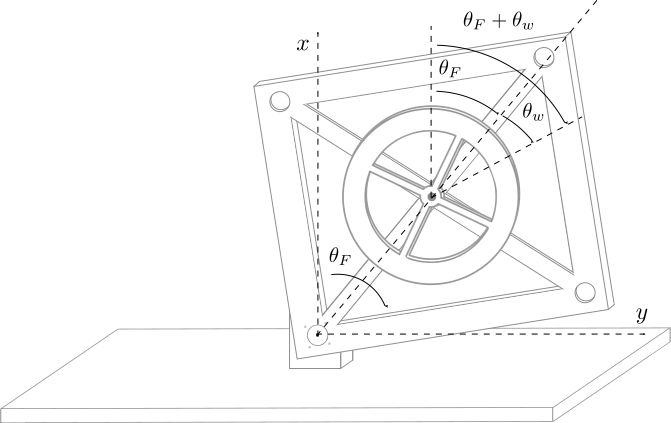
\includegraphics[scale=0.6]{figures/mechanicalSystem}
 \caption{Mechanical drawing of the Cubli, including angle coordinate system conventions}
 \label{cubliMechanical}
\end{figure}

%As shown in \figref{cubliMechanical}, 
In the next section, a complete model of the given setup is derived from Newton's Second Law of motion and rotation.
\input{chapters/chapter5/bDerivationOfModel.tex}      %-------- Derivation
\section{Linearization of the Model}
Now that a model of the Cubli frame is put forth in \eqref{FrameEqFinal}, it is apparent that the system is nonlinear due to the term including \si{sin(\theta_F)}. In order to proceed with a simulation and controller design, it is convenient to first linearize the model. This is done by use of a Taylor series approximation.

Based on \eqref{FrameEq3} the system is described in an operating point, around which it varies with \si{\Delta \theta_F}.
%
\begin{flalign}
	\si{(J_F+m_w \cdot {l_w}^{2}) (\ddot{\theta}_F + \Delta \ddot{\theta}_F )} &= \si{- B_F \cdot (\dot{\theta}_F + \Delta \dot{\theta}_F) }   \nonumber\\
	&\ \ \ \ \si{+ (m_F \cdot l_F + m_w \cdot l_w) \cdot g \cdot sin(\theta_F + \Delta \theta_F)} \nonumber\\
	&\ \ \ \ \si{- \tau_M + B_w \cdot \dot{\theta}_w}  \unit{N \cdot m}\\
	\eq{(J_F+m_w \cdot {l_w}^{2}) (\ddot{\theta}_F + \Delta \ddot{\theta}_F )}{ f( (\dot{\theta}_F + \Delta \dot{\theta}_F), \ (\theta_F + \Delta \theta_F), \ (\tau_m + \Delta \tau_m),\  (\dot{\theta}_w + \Delta \dot{\theta}_w) ) } \unit{N \cdot m}
\label{FrameEq4OperatingPoint}
\end{flalign}
%
The operating point is chosen to be \si{\theta_F = 0}, which corresponds to the frame being in upright position, see \figref{cubliMechanical}. Taking this into account and applying the Taylor series approximation yields the following.
%
\begin{flalign}
	\si{(J_F+m_w \cdot {l_w}^{2}) \Delta \ddot{\theta}_F } &= \cancelto{0}{\si{f( \dot{\theta}_F, \ \theta_F, \ \tau_m,\ \ddot{\theta}_w )}}   \nonumber\\
	&\ \ \ \ \si{+ \frac{\partial}{\partial \dot{\theta}_F} f\cdot \Delta \dot{\theta}_F + \frac{\partial}{\partial \theta_F} f\cdot \Delta \theta_F + \frac{\partial}{\partial \tau_m} f\cdot \Delta \tau_m + \frac{\partial}{\partial \dot{\theta}_w} f\cdot \Delta \dot{\theta}_w } \unit{N \cdot m}
\label{FrameEq4OperatingPointZero}
\end{flalign}

All the higher order derivatives are discarded due to their negligible impact on the system when it is near the operating point.
%
\begin{flalign}
	\si{(J_F+m_w \cdot {l_w}^{2}) \Delta \ddot{\theta}_F } &= \si{-B_F \Delta \dot{\theta}_F +  ( m_F \cdot l_F + m_w \cdot l_w ) g \cdot} \cancelto{1}{\rule{0cm}{.4cm} \si{  cos(\theta_F)}} \si{\Delta \theta_F} \where{\theta_F = 0} \nonumber\\
	&\ \ \ \ \si{- \Delta \tau_m + B_w \Delta \dot{\theta}_w } \unit{N \cdot m}\\
	\eq{(J_F+m_w \cdot {l_w}^{2}) \Delta \ddot{\theta}_F }{-B_F \Delta \dot{\theta}_F +  ( m_F \cdot l_F + m_w \cdot l_w ) g \cdot \Delta \theta_F - \Delta \tau_m + B_w \Delta \dot{\theta}_w } \unit{N \cdot m}
\label{FrameEq4TaylerApprox}
\end{flalign}
%
\Eqref{FrameEq4TaylerApprox} shows the final linearized model.

\begin{figure}[H] 
	\centering 
	\includegraphics[scale=1.5]{figures/linearizationPoint}
	\caption{Sketch of linearization for the Cubli frame angels.}
	\label{LinearizationSketch}
\end{figure} 

Due to the linearization of the model there will be an point where the controller will no longer be able to catch the frame, because it cannot predict the forces on the frame anymore. In the sketch (see \figref{LinearizationSketch}) the area where the controller will work is indicated by the green area.    %-------- Linearization
\input{chapters/chapter5/dBlockDiagram.tex}    		    %-------- Block Diagram

%---------- Chapter 6 ---------------------------------------- Plant Analysis
\chapter{Plant Analysis}

Once the model of the system has been described, a further analysis can be done. It includes the acquisition and estimation of the parameters, the model testing and the stability analysis.

\section{Acquisition of Parameters}\label{sec:Param}

A method to obtain the parameters from the wheel (mass, distance from its center to the pivoting point of the frame, inertia with respect to its center of rotation and friction) is provided in \appref{app:wheelParameters}. However, these parameters should remain constant and they have been obtained by previous project runners, it is chosen to use these known parameters\cite{SVJohansen}.

\begin{table}[H]
	\begin{tabular}{|l|l|p{3cm}|}
		\hline %-----------------------------------------------------------------------------------
		\textbf{Parameter} &\textbf{Value} &\textbf{Units}\\
		\hline %-----------------------------------------------------------------------------------
		\si{m_w}         & \si{0,222}       &kg\\
		\hline
		%-----------------------------------------------------------------------------------
		\si{l_w}         & \si{0,093}       &m\\
		\hline %-----------------------------------------------------------------------------------
		\si{J_w}         & \si{0,601 \cdot 10^{-3}}	&\si{kg \cdot m^2}\\
		\hline  
		%-----------------------------------------------------------------------------------
		\si{B_w}         & \si{17,03 \cdot 10^{-6}}       &N \si{\cdot m \cdot s \cdot rad^{-1}}\\
		\hline
	\end{tabular}
	\caption{Parameters of the wheel}
	\label{ParametersWheel}
\end{table}

However, the rest of the parameters (\si{m_F, l_F, J_F\ and\ B_F}) must be found out. This is due to the addition of the electronics to the frame, which were not there when the previous groups tests were made.

\subsection{Mass of the Frame}
The first one to find is the mass of the frame, which can be measured by weighing the setup without the base and substracting the known mass of the wheel. This gives a mass of \si{0,548\ kg}.

\subsection{Center of Mass of the Frame}
The new center of mass can be found hanging the frame from different corners and measuring the deviation angle from the vertical position in every direction. This gives a center of mass which can be seen in \figref{centerOfMassDiagram}. 
\begin{figure}[H]
	\centering
	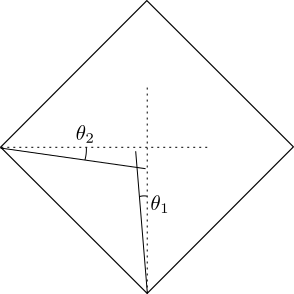
\includegraphics[scale=0.6]{figures/centerOfMassDiagram}
	\caption{Location of the center of mass, where \si{\theta_1=0,043\ rad\ and\ \theta_2=0,078\ rad}}
	\label{centerOfMassDiagram}
\end{figure}


The new point is not in the vertical line as it was assumed in the model, but this can be solved correcting the offset in the calculation of the angle inside the control loop and taking this new point as the equilibrium one. 

The new \si{l_F} can then be obtained projecting the center of mass onto the vertical line, resulting in \si{8,498\ cm}.

\subsection{Inertia and Friction of the Frame}
In the previous sections parameters have been found, however, some critical parameters were given from a previous project. When these parameters were found, the Cubli had another mass, due to some physical modifications of the platform, which were performed after the refereed project. The critical parameters are \si{J_F} and \si{B_F}. If the model is compared with reality, as seen on \figref{InitialModelParameterCompare}, it is evident that some further tuning of the parameters is needed.

\begin{figure}[H] 
	\centering
	\includegraphics[width=.7\textwidth]{figures/InitialModelParameterCompare}
	\caption{A comparison of the model simulation and the initially given parameters (\si{J_F=6,08 \cdot 10^{-3}\ kg \cdot m^2\ and\ B_F=5,32 \cdot 10^{-3}\ m \cdot s \cdot rad^{-1}})}
	\label{InitialModelParameterCompare}
\end{figure}

This problem can be solved using optimization, which is the subject of the proceeding section.\fxnote{Include Senstools manual and reference it here}  	    %-------- Parameter Estimation
\section{Model Testing}
Substituting all the constants of \eqref{2ndCubliTransferFunction} with the parameters of the real model results in the final transfer function of the system.
%
\begin{flalign}
	\eq{G(s)}{\frac{-148,8 \cdot s}{s^3 + 1,177 \cdot s^2 - 98,19 \cdot s - 2,783}} &\nonumber\\
	\label{RealCubliTransferFunction}	
\end{flalign}
%
Using \eqref{RealCubliTransferFunction} it is possible to simulate the response of the system to a step input and compare it with the response of the simulation of the block diagram. This is done to verify that the block diagram is in fact showing the system described in \eqref{RealCubliTransferFunction}, as seen in \figref{stepComparison}.

\begin{figure}[H] 
	\centering 
	\includegraphics[scale=0.65]{figures/stepComparison}
	\caption{Step response comparison between the transfer function from \eqref{RealCubliTransferFunction} and the block diagram from \figref{cubliSimulink}. The conclusion form this is the blockdiagram of the system was made correctly..}
	\label{stepComparison}
\end{figure}


In \figref{LinearizedVSNonlinear}, the effect of the linearization is apparent. In the simulation the frame is placed in upright position very slightly off \si{0\ rad}. The small deviation from \si{0\ rad} is applied in the last plant feedback, see \figref{cubliSimulink}. If, in the simulation, the model is started out at exactly \si{0\ rad}, it will balance in upright position.
\Figref{LinearizedVSNonlinear} shows the behavior around the frame's pivot point and does not include the platform itself. For this reason, the simulation allows for the frame to fall down and act as a normal pendulum. The nonlinear model shows how the pendulum dampens around its natural equilibrium point, while the linear model keeps increasing the angle.
However, in reality the platform blocks the frame's path, and so, it can only ever turn \si{45 ^\circ} to either side, that is, \si{\frac{\pi}{4}\ rad \approx 0,79\ rad}.
%
\begin{minipage}{\linewidth}
  \begin{minipage}{0.5\linewidth}
    \begin{figure}[H]
    	\includegraphics[scale=.55]{figures/LinearizedVSNonlinear}
    	\centering
  		\captionsetup{justification=centering}
  		\captionof{figure}{Simulation of the linearized model compared to the nonlinear model.}
  		\label{LinearizedVSNonlinear}
  	\end{figure}
  \end{minipage}
  %	\hspace{0.03\linewidth}
  \begin{minipage}{0.5\linewidth}
  	\begin{figure}[H]%\vspace{-7mm}
  		\includegraphics[scale=.55]{figures/LinearizedVSNonlinearZoom}
  		\centering
  		\captionsetup{justification=centering}
  		\captionof{figure}{Zoom of \figref{LinearizedVSNonlinear} to show the deviation of the linearization from the nonlinear model.}
  		\label{LinearizedVSNonlinearZoom}
  	\end{figure}
  \end{minipage}
\end{minipage}

From \figref{LinearizedVSNonlinear} and \figref{LinearizedVSNonlinearZoom}, the linearized model is considered a good approximation of the system's behavior in the operational region of \si{\pm 0,79\ rad}, since the error committed is no more than \si{0,01\ rad} at this point.

To further investigate the model, another test is made, see \appref{app:fallResponseAppendix}, to determine weather the fall response of the nonlinear model and the real system matches.

\begin{minipage}{\linewidth}
	\begin{minipage}{0.5\linewidth}
		\begin{figure}[H]
			\includegraphics[scale=.55]{figures/FallTestComparison}
			\centering
			\captionsetup{justification=centering}
			\captionof{figure}{Comparison of test and nonlinear model of frame falling from equilibrium position}
			\label{FallTestComparison}
		\end{figure}%\vspace{-5mm}
	\end{minipage}
%	\hspace{0.03\linewidth}
	\begin{minipage}{0.5\linewidth}
		\begin{figure}[H]%\vspace{-4mm}
			\includegraphics[scale=.55]{figures/FallTestComparison10deg}
			\centering
			\captionsetup{justification=centering}
			\captionof{figure}{Comparison of test and model of frame falling from initial condition \si{-0,174\ rad}}
			\label{FallTestComparison10deg}
		\end{figure}%vspace{-5mm}
	\end{minipage}
\end{minipage}

In \figref{FallTestComparison} the Cubli falls from equilibrium position given a very small impulse. When plotting the two data sets the time of the fall is aligned to see if the characteristics of the simulated fall matches reality.\\
To show that the simulation matches reality regardless the initial condition, the test is repeated starting from \si{-0,174\ rad} (\si{-10^\circ}) in both simulation and test, the result is shown in \figref{FallTestComparison10deg}.

%Hence the linearized model is used both for further analysis of the system and for controller design.
		      %-------- Model Analysis
\section{Stability Analysis}
The linearized model is considered valid within the discussed range of angles (\si{\pm 0,79\ rad}), so it can be used to do a deeper analysis on the behavior of the system. %This includes evaluations in frequency domain, s-domain and L(s)-domain.

%\subsection{Bode Diagram}
%The Bode diagram gives the frequency response of the system, in both magnitude and phase plots, as seen in \figref{bodeTF}.
%\begin{figure}[H] 
%	\centering 
%	\includegraphics[scale=0.65]{figures/bodeTF}
%	\caption{Bode diagram of the system}
%	\label{bodeTF}
%\end{figure} 
%
%The graph also provides information about the stability of the system, given by the gain and phase margins. 
%
%In this case the first one is just infinite because the phase never crosses \si{-180^o} or \si{180^o}. However, the phase margin is \si{-118^o}, which means that the phase has some margin before becoming unstable.
%
%Looking only at the Bode plot, the system may be seen as stable, but the inverted pendulum is known to be an unstable system, so further analysis has to be done.

\subsection{Root Locus}
The Root Locus plot gives information about the location of the poles and zeros in open loop, and how the poles in closed loop will change as the gain of the whole system increases.

As seen in \figref{rlocusCubli} and \figref{rlocusCubliZoom} the system has one zero \si{(s=0)}, and three poles \si{(s=-10,6130}, \si{s=-0,0283} and \si{s=9,3213)}. This means that the system is unstable as it has one pole in the Right Half Plane (RHP) and, moreover, as one of the branches never crosses over to the Left Half Plane (LHP), the system can not be controlled just with a proportional controller.

\begin{minipage}{\linewidth}
 	\begin{minipage}{0.45\linewidth}
 		\begin{figure}[H]
 			\includegraphics[scale=.56]{figures/rlocusCubli}
 			\centering
 			\captionsetup{justification=centering}
 			\captionof{figure}{Root Locus of the system}
 			\label{rlocusCubli}
 		\end{figure}
 	\end{minipage}
 	\hspace{0.03\linewidth}
 	\begin{minipage}{0.45\linewidth}
 		\begin{figure}[H]\vspace{4mm}
 			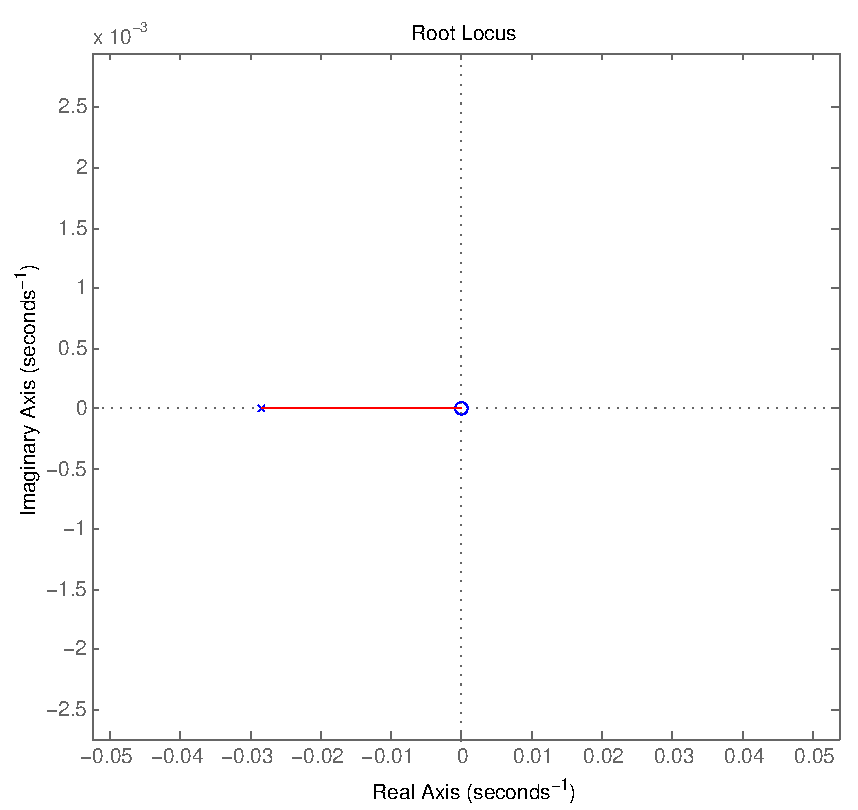
\includegraphics[scale=.56]{figures/rlocusCubliZoom}
 			\centering
 			\captionsetup{justification=centering}
 			\captionof{figure}{Zoom of \figref{rlocusCubli} from s=-0.04 to s=0.04}
 			\label{rlocusCubliZoom}
 		\end{figure}
 	\end{minipage}
\end{minipage}

\subsection{Nyquist Plot}
In any transfer function, the zeros of 1+L(s) (L(s) being the open loop function) become the poles of the closed loop system. That is why it is interesting to look at the Nyquist Stability Criterion, which can give information about this topic.

The number of zeros in the RHP of 1+L(s) (\si{Z_{RHP}}) is given by the number of poles of the L(s) (\si{P_{RHP}}) and the number of clockwise encirclements of the Nyquist plot around -1 (\si{N}) (a counterclockwise circle has a negative sign in this equation).
%
\begin{flalign}
	\eq{Z_{RHP}}{N+P_{RHP}} 
	&\nonumber\\
	\label{ZNP}
\end{flalign}
%
For the system to be stable (\si{Z_{RHP}}) has to be zero, which means that there is no pole of the close loop function in the RHP.

In the case of this plant, the number of poles of L(s)=G(s) in the RHP is one and there are no encirclements of -1 in the Nyquist plot (\figref{nyquistCubli}). That results in one zero in the RHP. As this zero will be a pole in the closed loop, the system is confirmed as unstable.

\begin{figure}[H] 
	\centering 
	\includegraphics[scale=0.6]{figures/nyquistCubli}	
	\caption{Nyquist plot of the plant}
	\label{nyquistCubli}
\end{figure}			        %-------- Stability Analysis

%---------- Chapter 7 ---------------------------------------- Requirements
%\chapter{Requirements}\label{chap:requirements}

%%% Part 2 %%%
\part{Design \& Implementation}
%---------- Chapter 8 ---------------------------------------- Control
\chapter{Controller Design}\label{chap:controllerDesign}
The controller design is a very wide field that goes from classic linear PID controllers to more advance techniques that use numerical optimization.

In this section, different types of linear controllers are presented and analyze in order to check if they are valid for the particular case of the Cubli. 
\section{Proportional Controller}\label{chap:pController}
Although a proportional controller can not be the final solution to balance the Cubli, it can be used to do a first approximation to the behavior of the system in closed loop.

The comparison between both responses, the simulated and the real one, with a contoller of gain 10 can be seen in \figref{closedLoopResponse}. 

\begin{figure}[H] 
	\centering 
	\includegraphics[scale=0.6]{figures/closedLoopResponse}	
	\caption{Behavior of the closed loop function with a proportional controller and a reference of 0 rad}
	\label{closedLoopResponse}
\end{figure}
It is clear that the closed loop function has an unstable response when a reference of 0 rad is required.
			      %-------- P Controller

%%% Part 3 %%%
\part{Test \& Conclusion}
%\input{chapters/aAcceptanceTest/AcceptanceTest}
%\chapter{Conclusion}

The aim of this project was to work with an unstable nonlinear system and be able to construct an appropriate model and design a controller capable of balancing it around equilibrium position.

First, a pre-analysis of the system has been made, starting from a description of all the components present in the given setup. It also included the derivation of the equations that describe the dynamics and the description of the system in s-domain. Then the parameters of the setup have been found, both with measurements and with an estimation using optimization, to be able to analyze the behavior of the system and compare it with the real model.

Afterwards, a controller has been designed to balance the Cubli in upright position using root locus. It has been shown necessary to control both the angular position of the frame and the velocity of the wheel so it was decided to use a state space approach.

It was also a requirement to be able to change the angle of the baseplate, which means that the calculation of the angle had to be independent of the inclination. A very convenient option was to use built-in sensors for this purpose, so the final chosen solution was to use an IMU present on the setup and calculate the angle through a complementary filter.

Finally, some acceptance tests have been performed to ensure that the final controlled system was able to accomplish the requirements and, similarly, a further analysis has been carried out to check other capabilities of the Cubli.

In conclusion, a control system that can balance the Cubli in upright position independently of the angle of the baseplate, within a reasonable range, has been designed, implemented and tested successfully within the requirements.

%\chapter{Discussion}

{\Large notes} \fxnote{delete this part its just to brainstorm what to write in this section}\\
- Placement of IMU\\
- Choice of Statspace variables for controller - minimize overshoot vs faster braking for wheel\\
- cut-off frequency of the complementary filter?\\
- 
- 


As already mentioned briefly in the complementary section the measurement from the accelerometer in the IMU could be improved by moving the sensor to a position where it would be influenced less by the acceleration of the frame but still be able to measure the angle of the frame. 



%%% Setup for Appendix and Bibliography %%%
\bookmarksetup{startatroot}
\addtocontents{toc}{\bigskip}
\newpage
\fancyhead[RO]{\color{aaublue}\small Appendix \nouppercase\rightmark} %even page - chapter title
\fancyhead[LE]{\color{aaublue}\small Appendix \nouppercase\rightmark} %uneven page - section title
\fancyhead[RE,LO]{}
\titleformat{\section}[hang]{\Large\bfseries}{\thesection\hsp\textcolor{aaublue}{|}\hsp}{0pt}{\Large\bfseries}
\renewcommand{\thechapter}{\Alph{chapter}}
\setcounter{chapter}{0}

%%% Appendix %%%
\part*{Appendix}
\addcontentsline{toc}{chapter}{Appendix}

%---------- Appendix A ---------------------------------------- 
\chapter{Potentiometer Angle Resolution}\label{app:potentiometerRes} 
\textbf{Name: Group 630}\\
\textbf{Date: 15/03 - 2016}

\subsubsection{Purpose}
Finding the resolution needed for the conversion of potentiometer voltage to angles, along with possible offsets.

\subsubsection{Setup}
\begin{figure}[H]
  \centering
	\includegraphics[scale=1]{figures/LabSetupRangeTest.pdf}
	\caption{Setup diagram}
	\label{LabSetupRangeTest2}
\end{figure}\vspace{-5mm}

\subsubsection{List of Equipment}
\begin{table}[H]
	\begin{tabular}{|l|l|p{4.3cm}|}
		\hline%------------------------------------------------------------------------------------------------------------
		\textbf{Instrument}                                  &  \textbf{AAU-no.}  &  \textbf{Type}                       \\
		\hline%------------------------------------------------------------------------------------------------------------
		Oscilloscope                                         &  61604             &  Agilent 54621A		                   \\
		\hline%------------------------------------------------------------------------------------------------------------
		Dedicated Power Supply of Cubli \small{(24 V - 3 A)} &                    &  XP Power, AEB70US24                 \\
		\hline%------------------------------------------------------------------------------------------------------------
		Probe                                          &                &   1:1   \\
		\hline%------------------------------------------------------------------------------------------------------------
	\end{tabular}
\end{table}

\subsubsection{Procedure}
\begin{enumerate}
  \item Make the setup with connections as seen on \figref{LabSetupRangeTest}, with ground on the brown cable and signal on yellow cable of the potentiometer.
  \item Set the oscilloscope on rolling and calibrate so that the full range of the frame movement can be captured on the display.
  \item Balance the frame in upright equilibrium position.
	\item Move the frame to the left position, hold for a brief duration, then move it over to the right position.
	\item Once both the equilibrium, leftmost and rightmost positions are captured on the screen, pushing the stop-button on the scope, to hold keep the measurement.
	\item Save the data to the floppy-disk as a CSV file.
\end{enumerate}

\subsubsection{Results}
\begin{figure}[H] 
	\centering 
	\includegraphics[scale=0.7]{figures/TestPotentiometerResolution}
	\caption{Raw test data plot, Volt over time.}
	\label{comparisonRealModel}
\end{figure}

%---------- Appendix B ---------------------------------------- 
\chapter{Vertical Initial Condition Response}\label{fallResponseAppendix} 
\textbf{Name: Group 630}\\
\textbf{Date: 17/03 - 2016}

\subsubsection{Purpose}
Find the fall response of the frame from the vertical position, \si{\theta_F=0}\fxnote{might change depending on what is decided as the "real" 0 because of potmeter offset}, and from a \si{10^\circ}\fxnote{Might chance depending on data } tilted position.
Data is used to compare the measured response and the simulation given by the theoretical nonlinear model.


\subsubsection{Setup}
The wheel is being held in a fixed position with a strip tied to it and the frame. The probe chosen is a 1:1 and is connected to the potentiometer with probe to yellow cable and ground clamp to brown cable. The power supply has to be turned on in order to get readouts from the potentiometer. A sponge is placed on the rubber pad in order to damp the impact of the frame.
\begin{figure}[H]                                   
	\centering                                        
	\includegraphics[scale=0.08]{figures/stepResponseSetup}
	\caption{Picture of the setup for the fall-response test}
	\label{stepResponseTestPicture} 
\end{figure}              

\subsubsection{List of Equipment}
\begin{table}[H]
	\begin{tabular}{|l|l|p{4cm}|}
		\hline%------------------------------------------------------------------------------------
		\textbf{Instrument}                        &  \textbf{AAU-no.}  &  \textbf{Type}       \\
		\hline%------------------------------------------------------------------------------------
		Cubli setup                              &               &  		  \\
		\hline%------------------------------------------------------------------------------------
		Oscilloscope                              &  61604             &  Agilent 54621A		  \\
		\hline%------------------------------------------------------------------------------------
		Dedicated Power Supply of Cubli \small{(24 V - 3 A)} &               &  XP Power, AEB70US24 \\
		\hline%------------------------------------------------------------------------------------
		Probe 1:1                &  TBD            &          TBD   \\
		\hline%------------------------------------------------------------------------------------
		Sponge               & 5P0N63             &              \\
		\hline%------------------------------------------------------------------------------------
	\end{tabular}
\end{table}
fix of table\fxnote{find the probe used} 
\subsubsection{Procedure}
\begin{enumerate}
	%\item Turn on the power supply
	\item Keep the Cubli in the starting position (\si{0^\circ} or \si{10^\circ})
	\item Let the Cubli fall over
	\item Use the oscilloscope to measure the voltage changes in the potentiometer and save them
	\item Take the measurements and plot them in Matlab
	%\item Plot the result of the simulations in the same figure and compare them
\end{enumerate}


\subsubsection{Results}
Data from the test is presented in a graph showing the voltage measured, and in a graph with the voltage converted to radians.
The data is available as a .csv file on the CD\fxnote{Make sure this is put into the CD folder for copying}

\small\textbf{Fall response starting from \si{0^\circ}}

\begin{minipage}{\linewidth}
	\begin{minipage}{0.45\linewidth}
		\begin{figure}[H]
			\includegraphics[scale=.53]{figures/FallVolt}
			\centering
			\vspace{-.4cm}
			\captionsetup{justification=centering}
			\captionof{figure}{Raw data taken from the potentiometer}
			\label{FallVolt}
		\end{figure}\vspace{-5mm}
	\end{minipage}
	\hspace{0.03\linewidth}
	\begin{minipage}{0.45\linewidth}
		\begin{figure}[H]
			\includegraphics[scale=.53]{figures/FallRad}
			\centering
			\vspace{-.4cm}
			\captionsetup{justification=centering}
			\captionof{figure}{Angular position of the frame}
			\label{FallRad}
		\end{figure}\vspace{-5mm}
	\end{minipage}
\end{minipage} \fxnote{Look at the layout of picture of data placement}

\small\textbf{Fall response starting from \si{10^\circ}}

\begin{minipage}{\linewidth}
	\begin{minipage}{0.45\linewidth}
		\begin{figure}[H]
			\includegraphics[scale=.53]{figures/tenDegFallVolt}
			\centering
			\vspace{-.4cm}
			\captionsetup{justification=centering}
			\captionof{figure}{Raw data taken from the potentiometer}
			\label{tenDegFallVolt}
		\end{figure}\vspace{-5mm}
	\end{minipage}
	\hspace{0.03\linewidth}
	\begin{minipage}{0.45\linewidth}
		\begin{figure}[H]

			\includegraphics[scale=.53]{figures/tenDegFallRad}
			\centering
			\vspace{-.4cm}
			\captionsetup{justification=centering}
			\captionof{figure}{Angular position of the frame}
			\label{tenDegFallRad}
		\end{figure}\vspace{-5mm}
	\end{minipage}
\end{minipage} \fxnote{Look at the layout of picture of data placement}
fix\fxnote{link the correct pictures for the 0 degree experiment}


%The result of the experiment (\figref{comparisonRealModel}) shows that the response of the real system has several differences with the one from the simulation.
%
%The fist one is the presence of oscillations in the real response curve. This behavior is due to a small bounce that the frame does when it reaches the base.
%
%Another one is the final position of the frame, but it is due to the existence of a piece of foam at this position in the real case (to avoid the Cubli to hit the base).
%
%The other main difference is the shape of the curve, since the simulation is slower than the real case.

\subsubsection{Note}

There can be observed some bouncing in the data when the frame reaches the lower position due to the presence of the sponge.
Because of the sponge used as a cushion, to dampen the impact of the Cubli, there can be observed some bouncing in the data when the frame reaches the outer position.

The conversion from voltage to radians is based upon the test done in appendix X\fxnote{ADD reference to potentiometer test and the math behind the scaling}





%----------Appendix C ---------------------------------------- 
\chapter{Pendulum Behavior Test}\label{app:impulseResponseAppendix} 

\textbf{Name: Group 630}\\
\textbf{Date: 16/03 - 2016}

\subsubsection{Purpose}
Observing the behavior of the Cubli when hanging upside down. Data is then used to estimate some of the parameters of the Cubli.

\subsubsection{Setup}
The Cubli is put upside down under a table with 2 clamps placed at each side of the bottom plate of the Cubli setup.
The wheel is being held in a fixed position with a strip tied to it and the frame. The probe chosen is a 1:1 and is connected to the potentiometer with probe to yellow cable and ground clamp to brown cable. The power supply has to be connected, and turned on, to the Cubli in order to get readouts from the potentiometer.
\begin{figure}[H] 
	\centering 
	\includegraphics[scale=0.2]{figures/impulseResponseSetup2}
	\caption{The Cubli setup hanging upside down beneath a table during the impulse response test}
	\label{impulseResponseTestPicture}
\end{figure} 

\subsubsection{List of Equipment}
\begin{table}[H]
	\begin{tabular}{|l|l|p{4.3cm}|}
		\hline%------------------------------------------------------------------------------------
		\textbf{Instrument}                        &  \textbf{AAU-no.}  &  \textbf{Type}       \\
		\hline%------------------------------------------------------------------------------------
		Oscilloscope                              &  61604             &  Agilent 54621A		  \\
		\hline%------------------------------------------------------------------------------------
		Dedicated Power Supply of Cubli \small{(24 V - 3 A)} &               &  XP Power, AEB70US24 \\
		\hline%------------------------------------------------------------------------------------
		Probe               &             		&          1:1  \\
		\hline%------------------------------------------------------------------------------------
		2x Clamp                &  			            &          							   \\
		\hline%------------------------------------------------------------------------------------
	\end{tabular}
\end{table}

\subsubsection{Procedure}
\begin{enumerate}
	%\item Turn on the power supply
	\item Place the setup upside-down and place the frame touching the base.
	\item Let the Cubli fall and swing until it stops.
	\item Use the oscilloscope to measure the changes in the potentiometer.
	\item Collect all the data and plot it in Matlab.	
\end{enumerate}

\subsubsection{Results}
The results of the experiment can be seen in \figref{PendVolt} and \figref{PendRad}. The second graph is obtained using the conclusions from \appref{app:potentiometerRes} explained in Section \ref{sec:Sensors}.

\begin{minipage}{\linewidth}
	\begin{minipage}{0.45\linewidth}
		\begin{figure}[H]
			\includegraphics[scale=.53]{figures/PendVolt}
			\centering
			\vspace{-.4cm}
			\captionsetup{justification=centering}
			\captionof{figure}{Raw data taken from the potentiometer}
			\label{PendVolt}
		\end{figure}%\vspace{-5mm}
	\end{minipage}
	\hspace{0.03\linewidth}
	\begin{minipage}{0.45\linewidth}
		\begin{figure}[H]\vspace{-4mm}
			\includegraphics[scale=.53]{figures/PendRad}
			\centering
			\vspace{-.4cm}
			\captionsetup{justification=centering}
			\captionof{figure}{Angular position of the frame}
			\label{PendRad}
		\end{figure}%\vspace{-5mm}
	\end{minipage}
\end{minipage}

\subsubsection{Note}
During this experiment it was observed that if the frame was released from the left position (the right upper side on \figref{impulseResponseTestPicture} since the Cubli is upside down), the frame would hit the rubber pad on the other side. This behavior was not observed when releasing the Cubli from the right position (left upper corner).



%---------- Appendix D ---------------------------------------- Test Title
%\input{appendix/dTest.tex}

%%% Bibliography %%%
\printbibliography

%%% To Do List %%%

\end{document}
